\chapter{Introduction to Bioinformatics}
\label{chap:intro}

This chapter offers an overview of the bioinformatics field, focusing on key molecular biology concepts needed in the context of this thesis. It covers proteins, their sequences and structures, ligands, binding sites (including cryptic binding sites), major biological databases and file formats, and widely used tools for visualization, binding site prediction, and structural analysis.

\section{Proteins, Ligands, and Amino Acids}
\label{sec:proteins}

\textbf{Proteins} are vital macromolecules involved in numerous biological functions, such as catalyzing biochemical reactions, offering structural support, and regulating cellular activities \cite{cooper2022cell}. They consist of \textbf{amino acids} connected by \textbf{peptide bonds}, forming \textbf{polypeptide chains}. Amino acids are molecules containing an amino group (\(-NH_2\)), a carboxyl group (\(-COOH\)), and a unique side chain (\(R\) group) that determines the amino acid's properties. The individual amino acid units within the polypeptide chain are referred to as \textbf{residues}, a term that may be used interchangeably with amino acids throughout this thesis. The sequence of these amino acids in a polypeptide chain is known as the \textbf{primary structure} of a protein. The sequence of the protein determines its function \cite{nelson2008lehninger}, \cite{voet2010biochemistry}. There are \textbf{20 standard amino acids}, each possessing distinct characteristics that affect protein folding and interactions with other molecules. While many non-standard amino acids are used in drug discovery and development \cite{dumas2015designing}, this thesis will primarily consider the 20 standard amino acids that form the basic building blocks of proteins.

\begin{figure}[ht]
    \centering
    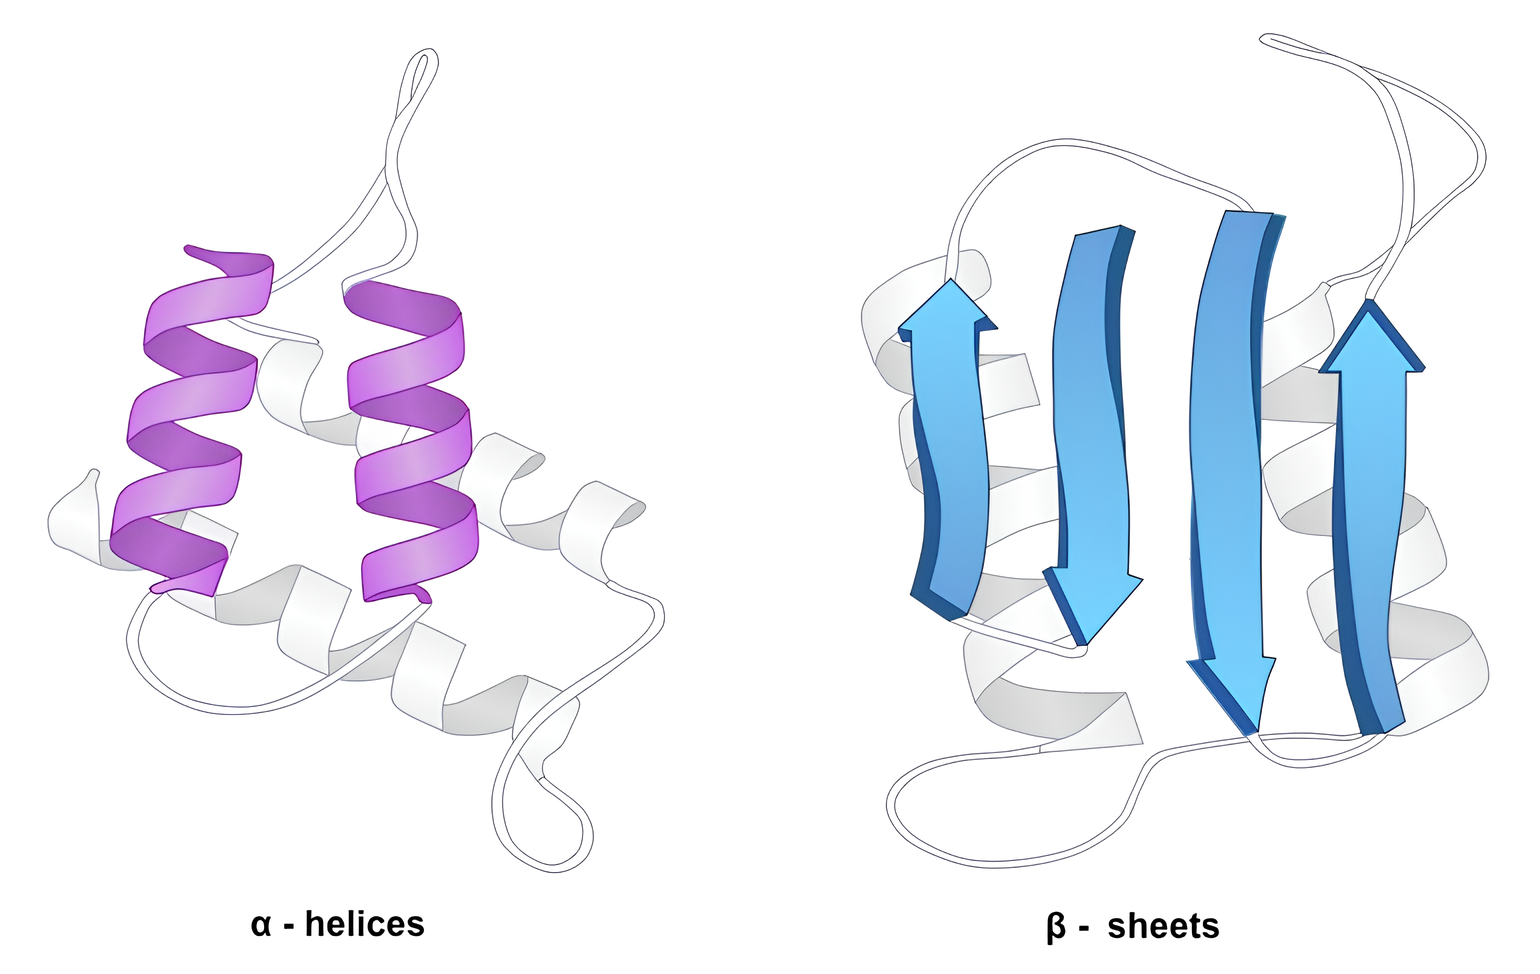
\includegraphics[width=0.8\textwidth]{img/ah_bs.png}
    \caption{Illustration of an alpha helices and a beta sheets, the two most common types of protein secondary structure. Adapted from an image by BioNinja~\cite{alphabetapicture}.}
    \label{fig:alpha-beta}
\end{figure}

The second level of protein structure is the \textbf{secondary structure}, which refers to local folding patterns within the polypeptide chain. The most common secondary structures are \textbf{alpha helices} and \textbf{beta sheets}, as shown in Figure~\ref{fig:alpha-beta}. These structures arise from hydrogen bonding between the backbone atoms of the amino acids, stabilizing the overall protein structure. All proteins also have a \textbf{three-dimensional (3D) structure}, also known as \textbf{tertiary structure}, which is crucial for their function \cite{nelson2008lehninger}, \cite{voet2010biochemistry}.

The secondary and tertiary structures are determined by the interactions between the side chains of the amino acids, including hydrophobic interactions, hydrogen bonds, ionic bonds, and disulfide bridges. The final level of protein structure is the \textbf{quaternary structure}, which refers to the assembly of multiple polypeptide chains into a functional protein complex \cite{nelson2008lehninger}, \cite{voet2010biochemistry}.

The tertiary and quaternary structures of proteins are determined through experimental methods such as X-ray crystallography and nuclear magnetic resonance (NMR) spectroscopy \cite{berman2000protein}. However, with the rise of deep learning and artificial intelligence, it is now also possible to predict protein structures from their amino acid sequences with remarkable accuracy. The most notable example is AlphaFold \cite{jumper2021highly}, \cite{abramson2024accurate}, a deep learning model developed by DeepMind that has achieved remarkable accuracy in predicting protein structures and has been widely adopted in the field of bioinformatics. AlphaFold also provides a per-residue confidence metric called the predicted Local Distance Difference Test (plDDT) score\footnotemark[1], which indicates the reliability of the predicted atomic positions. In recognition of the profound impact of these advances, the Nobel Prize in Chemistry was awarded in 2024 for the development of methods for the prediction of protein structures using artificial intelligence \cite{abriata2024nobel}. Other notable tools introduced in the past months include Boltz-2 \cite{passaro2025boltz2} and Chai-1 \cite{chai2024chai}. Today, predicted structures often closely match experimental results, as illustrated in Figure~\ref{fig:alphafold-vs-exp}.

\footnotetext[1]{The predicted Local Distance Difference Test (plDDT) score is a per-residue confidence metric output by AlphaFold, indicating the reliability of the predicted atomic positions; higher values suggest greater confidence. In the color scheme, blue indicates the most confident regions, while orange/yellow depict less confident regions.}

\begin{figure}[ht]
    \centering
    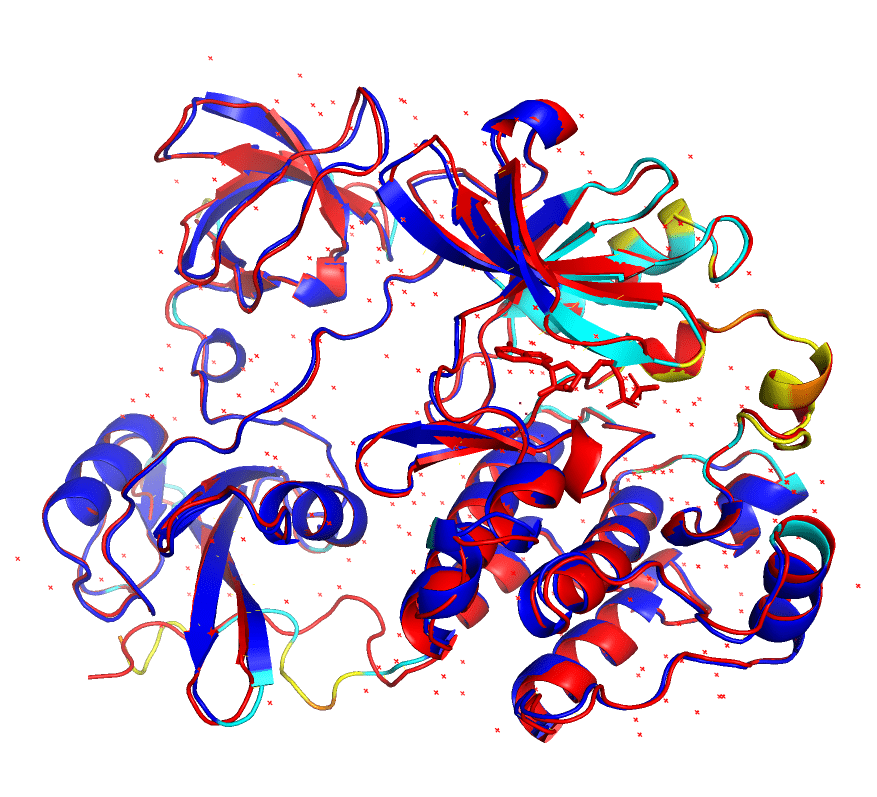
\includegraphics[width=0.8\textwidth]{img/alphafold_vs_exp.png}
    \caption{Comparison of AlphaFold predicted structure and experimental structure of the protein 2SRC (Crystal Structure of Human Tyro\-sine-Protein Kinase C-SRC, in Complex with AMP-PNP). The predicted structure is shown in blue to yellow colors (depicting the plDDT score), while the experimental structure is shown in red. The two structures are nearly identical after the alignment, demonstrating the accuracy of AlphaFold predictions. Image created in PyMOL.}
    \label{fig:alphafold-vs-exp}
\end{figure}
\par

Protein function is largely determined by interactions with other molecules, known as ligands. These may be small molecules, ions, RNA molecules, lipids, saccharides, or other molecules that bind to specific regions, often resulting in conformational changes that lead to different functions. Such interactions are crucial for processes like enzymatic catalysis, signal transduction, and immune response. In drug discovery, identifying and characterizing these sites is important, with computational approaches aiding both new therapeutic development and drug repurposing \cite{konc2019binding}. Additionally, de novo protein design allows for the creation of proteins with tailored functions, often guided by predictive tools such as AlphaFold before experimental testing \cite{huang2016coming}.

\section{Cryptic Binding Sites (CBSs)}
\label{sec:binding-sites}

\textbf{Binding sites} are distinct regions on a protein where ligands can bind and interact. These sites typically manifest as cavities or grooves on the protein surface and are frequently linked to conformational changes that influence protein function. Proteins with a ligand bound are termed \textbf{holo} conformations, while those lacking a ligand are called \textbf{apo} conformations. In holo conformations, the binding site is defined by the ligand’s position, whereas apo conformations may contain several potential binding sites, also commonly known as \textbf{pockets}.

\textbf{Cryptic binding sites (CBSs)} are regions on proteins that are not visible or accessible in the unbound (apo) structure but can form and become available for ligand binding following conformational changes. These sites typically appear only after ligand interaction or other molecular events that induce structural rearrangements.

A key concept in the study of CBSs is the use of \textbf{apo–holo protein pairs}. An \textbf{apo structure} refers to a protein in its unbound state (without a ligand), while a \textbf{holo structure} is the same protein bound to a ligand. Comparing these paired structures allows researchers to identify binding sites that are only present or accessible in the holo form, thus revealing cryptic sites.

Computational methods such as CryptoBench \cite{vskrhak2025cryptobench} have been created to predict cryptic binding sites. A significant contribution in this area is CryptoSite \cite{cimermancic2016cryptosite}, which leverages known apo–holo protein pairs to identify CBSs, offering an alternative to time-consuming molecular dynamics simulations. Both of the methods will be covered in more detail in Section~\ref{sec:related-tools}.

\section{Databases and File Formats}
\label{sec:dbs-formats}

This section provides an overview of the key bioinformatics databases for protein structures and introduces the main file formats used in this field.

\subsection{PDB Archive and RCSB PDB}
\label{sec:rcsb-pdb}

The PDB (Protein Data Bank) Archive, often referred to simply as the "PDB database", is a comprehensive repository of 3D structural data for experimentally determined proteins, nucleic acids, and complex assemblies. It serves as a foundational resource for bioinformatics, with many machine learning and deep learning models relying on its data for training and validation. The archive is maintained by the wwPDB (Worldwide PDB) organization \cite{berman2003announcing}, which includes the RCSB PDB (Research Collaboratory for Structural Bioinformatics Protein Data Bank) \cite{berman2000protein}, PDBe (Protein Data Bank in Europe) \cite{velankar2010pdbe}, PDBj (Protein Data Bank Japan) \cite{kinjo2012protein}, and other members. 

The RCSB PDB (Research Collaboratory for Structural Bioinformatics Protein Data Bank) group offers a REST API for programmatic data access, which is publicly accessible at \url{https://www.rcsb.org/}. As of June 2025, the database contains over 238,000 structures.

Many organizations also maintain local, enriched copies of the PDB archive. The open sharing of structural data is encouraged, as it supports the development and improvement of computational models used throughout the scientific community \cite{callaway2025alphafold}.

\subsection{AlphaFold Database}
\label{sec:alphafold-db}

The AlphaFold Database \cite{varadi2024alphafold} contains over 200 million protein structures predicted by the AlphaFold model. While the majority of these structures have not been experimentally validated, those with high pLDDT scores are considered reliable. It is important to note that certain protein regions, known as intrinsically disordered regions, may exhibit low pLDDT scores due to their inherent flexibility and lack of stable structure. The database is publicly available at \url{https://alphafold.ebi.ac.uk/}.

\subsection{UniProt Database}
\label{sec:uniprot-db}

The UniProt database \cite{uniprot2025uniprot} is a comprehensive resource for protein sequences and functional information. Each protein is assigned a unique \textbf{UniProt accession} (also called \textbf{protein ID}), which serves as a standardized identifier for that specific protein. A single UniProt accession may correspond to multiple experimental structures in the PDB database, representing different conformations or states of the same protein, while typically having one predicted structure in the AlphaFold database. UniProt accessions are commonly used to link PDB and AlphaFold entries. UniProt is available at \url{https://www.uniprot.org/}. The main part of the UniProt database is the UniProt Knowledgebase (UniProtKB), which contains two sections: UniProtKB/Swiss-Prot, which includes manually curated entries with high-quality annotations, and UniProtKB/TrEMBL, which contains automatically annotated entries that have not yet been reviewed \cite{boutet2016uniprotkb}.

\subsection{PDB File Format}
\label{sec:pdb-format}

The PDB (Protein Data Bank) file format is a text-based format used to represent three-dimensional structures of biological molecules, primarily proteins and nucleic acids. It contains information about atom coordinates, connectivity, b-factors, and other structural details. Each PDB file should start with header lines providing metadata about the structure, such as the structure name, authors, methods used and additional comments. Then, the atomic coordinates are listed in a list of ATOM and HETATM records, which specify the atom type, residue name, chain identifier, residue sequence number, and the x, y, z coordinates of each atom in the structure. The PDB format might include information about secondary structure elements, such as helices and sheets \cite{westbrook2003pdb}. Some of the information might be ommited, especially in the case of working with structures generated by deep learning methods, such as RFDiffusion \cite{watson2023novo}. A single PDB file may contain multiple models representing distinct conformations of the same protein. It is worth noting that the PDB format is considered deprecated in favor of the more modern mmCIF format (covered in \ref{sec:mmcif-format}), though it remains widely used due to its simplicity and broad tool support.

\begin{figure}[H]
    \centering
    \lstinputlisting[caption={
        An edited example of a PDB file containing information about a protein structure generated by RFDiffusion.
    }]{code/rfdiff_example.pdb}
\end{figure}


\subsection{mmCIF File Format}
\label{sec:mmcif-format}

The mmCIF (Macromolecular Crystallographic Information File, also called PDBx) format is a more modern and flexible alternative to the PDB format, designed to overcome the limitations of the PDB format, especially for large structures \cite{bourne199730}. The PDB database, mentioned in Section~\ref{sec:rcsb-pdb}, has been transitioning to the mmCIF format for new entries. Although it is encouraged to use mmCIF for new structures, many existing tools and databases still rely on the PDB format thanks to its simpler format. Like PDB files, mmCIF files can also represent multiple conformations of the same structure.

\subsection{FASTA File Format}
\label{sec:fasta-format}

The FASTA file format is a widely used, text-based format for representing biological sequences, such as proteins or nucleic acids. Each sequence entry begins with a header line that starts with a ">" character, followed by a description or identifier. The sequence itself is written on the following lines, typically using single-letter codes. Multiple sequences can be included in a single FASTA file, each with its own header. While the header line is commonly present, it is technically optional, which allows easy creation of FASTA files \cite{lipman1985rapid}.

\begin{figure}[H]
    \centering
    \lstinputlisting[
        caption={
            An example of a FASTA file containing information about the 6A5J sequence (containing only 13 amino acids).
        },
        breaklines=true
    ]{code/fasta_example.fasta}
\end{figure}

\subsection{XTC File Format}
\label{sec:xtc-format}

The XTC (eXtended Trajectory Coordinate) file format is a binary format commonly used to store molecular dynamics simulation trajectories, especially in the GROMACS software package \cite{van2005gromacs}. It is widely used for efficiently storing large amounts of trajectory data, including atomic coordinates, velocities, and box dimensions, in a compressed binary format. In the context of bioinformatics, XTC files are often used to capture and analyze protein trajectory changes over time, enabling researchers to study conformational dynamics and structural transitions during simulations.

\section{Related Tools and Projects}
\label{sec:related-tools}

This section is dedicated to the most relevant tools and projects important for the work presented in this thesis.

\subsection{P2Rank and PrankWeb}
\label{sec:prankweb-p2rank}

P2Rank is a Groovy/Java based standalone tool for predicting binding sites in protein structures. The P2Rank algorithm is based on machine learning. The structure is covered with a grid of points on the protein's solvent accessible surface, and each point is assigned a score based on the likelihood of being a binding site based on the local environment of the point. Then, the points are clustered and ranked based on their scores. The pre-trained tool does not rely on any external databases nor templates. The method is widely adapted due to its reliable and accurate predictions and speed \cite{krivak2018p2rank}. Source codes for P2Rank are available at \url{https://github.com/rdk/p2rank}.

PrankWeb is a web-based interface for P2Rank, allowing simple access to the P2Rank method without the need to run and install the tool locally. It is available at \url{https://prankweb.cz/}. The web interface allows users to upload a PDB/mmCIF file and receive a visualization of the prediction of the binding sites with the predicted binding sites colored according to their scores. Moreover, PrankWeb allows the users to perform molecular docking using the predicted binding sites, which is a common post-processing step in drug discovery \cite{polak2025prankweb}, \cite{jakubec2022prankweb}, \cite{jendele2019prankweb}. The docking is performed using the AutoDock Vina \cite{trott2010autodock} software, which is a widely used tool for molecular docking.

The PrankWeb interface was a huge inspiration for the design of the web interface presented in this thesis as the goal is to provide a similar user experience, but with a focus on cryptic binding sites and its specific challenges.

\subsection{AHoJ}
\label{sec:ahoj}

AHoJ (Apo–Holo Juxtaposition) is a web application for retreiving and visualizing apo-holo pairs of proteins (See Section~\ref{sec:binding-sites}). This functionality is useful especially for cryptic binding site predictions, as it allows the users to find similar structures with possibly similar properties based on the predicted CBS \cite{feidakis2022ahoj}. The application is available at \url{https://apoholo.cz/}. Currently, AHoJ supports searching for apo-holo pairs only by PDB ID.

AHoJ is integrated within the CryptoShow interface as well. This will be covered in more detail in Section~\ref{sec:trajectory}.

\subsection{PyMOL}
\label{sec:pymol}

PyMOL is a powerful molecular visualization tool written in Python. The users might use it either as a standalone application or as a Python library. Thanks to its feature-rich API and UI, PyMOL is a common choice for researchers in structural biology and cheminformatics \cite{delano2002pymol}.

\subsection{Mol*}
\label{sec:molstar}

Mol* (also MolStar) is a TypeScript library for visualizing molecular structures directly in web browsers. Thanks to its modern architecture, the usage of WebGL and rich feature set, Mol* is nowadays a very popular choice for web-based molecular visualization tools \cite{sehnal2018mol}. Mol* also provides an online version of a molecular viewer, which is available at \url{https://molstar.org/viewer/} \cite{sehnal2021mol}. A highly-customized version of the viewer is also used in the CryptoShow interface, which will be covered in more detail in Section~\ref{sec:frontend}.

\begin{figure}[ht]
    \centering
    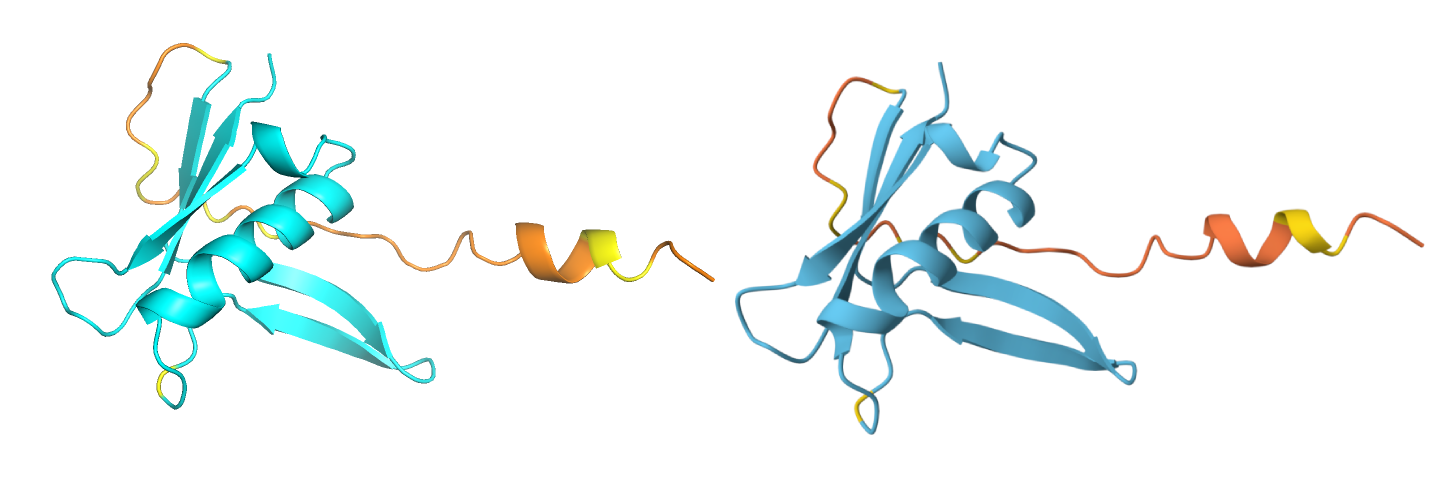
\includegraphics[width=\textwidth]{img/pymol-molstar.png}
    \caption{A comparsion of the PyMOL (left) and Mol* (right) molecular viewers showing the AlphaFold predicted structure of the protein AF\_AFQ9XWU9F1.}
    \label{fig:pymol-molstar}
\end{figure}

\subsection{CryptoBench}
\label{sec:cryptobench}

CryptoBench is a comprehensive benchmark dataset for training and evaluating CBSs prediction methods, built from a large set of apo–holo protein pairs and grouped by UniProt ID with predefined cross-validation splits. A part of the publication is dedicated to baseline evaluations, which show that a sequence-based neural network using protein language model embeddings outperforms state-of-the-art structure-based methods like PocketMiner \cite{meller2023predicting} and P2Rank \cite{krivak2018p2rank} across key metrics in terms of CBSs. The source codes for CryptoBench are available at \url{https://github.com/skrhakv/CryptoBench/} \cite{vskrhak2025cryptobench}.

The model used in CryptoBench (referred to as \textbf{CB-Model} in the context of this thesis) is able to predict cryptic binding sites when provided with ESM-2 embeddings \cite{lin2022language} of the protein sequence. The prediction capability represents one of the core functionalities of CryptoShow. More details about the CryptoBench method will be provided in Section~\ref{sec:prediction}.

\subsection{CryptoSite}
\label{sec:cryptosite}

CryptoSite is another tool designed to identify CBSs. By constructing a dataset of structurally defined apo–holo pairs, CryptoSite characterizes cryptic sites based on sequence, structure, and dynamics. Leveraging these insights, CryptoSite uses machine learning to predict cryptic sites with high accuracy, expanding the set of potentially druggable proteins. The tool has been applied to the human proteome, increasing the fraction of disease-associated proteins considered druggable. Experimental validation further demonstrates the practical use of CryptoSite. The web server is accessible at \url{https://modbase.compbio.ucsf.edu/cryptosite} \cite{cimermancic2016cryptosite}.

While CryptoSite is a valuable resource for cryptic binding site analysis and its web server remains available, its computational processes often take several days to complete, limiting its suitability for interactive use. In contrast, a primary goal of CryptoShow is to provide a fast and interactive experience, allowing users to obtain results within minutes. This need is underscored by the relatively low usage of CryptoSite; as of June 2025, only 10 jobs were submitted in the last 7 days. Also, the results of the CryptoSite jobs are available only for 7 days after the job completion.
